\begin{definition}
    $a_0, a_1, \ldots$~--- последовательность,
    тогда $\mathscr A(z) \coloneqq \sum\limits_{n=0}^{+\infty} a_nz^n$~---
    производящая функция.
\end{definition}

\begin{observation}
    Можем складывать, вычитать и не думать о сходимости.
\end{observation}

\begin{observation}
    Можем перемножать:

    \[
        \mathscr A(z) \mathscr B(z) = \sum\limits_{n=0}^{+\infty}
        c_nz^n
    \]

    где $c_n = a_0b_n + a_1b_{n-1} + \cdots + a_nb_0$.
\end{observation}

\begin{observation}
    Можем писать композицию $\mathscr A(\mathscr B(z))$
    если $b_0 = 0$, так как иначе
    приходится подставлять в формальный ряд
    какое-то значение.

    \[
        \mathscr A(\mathscr B(z)) = a_0 + a_1 \mathscr B(z) +
        a_2\mathscr B^2(z) + \cdots
        + a_k \mathscr B^k(z) + \cdots
    \]

    Чтобы посчитать конкретный коэффициент, достаточно
    вычислить конечный префикс ряда.
\end{observation}

\begin{observation}
    Можем писать формальное дифференцирование
    и интегрирование.
\end{observation}

\begin{definition}
    Произведение Адамара.

    $\mathscr A(z) = \sum a_nz^n$, $\mathscr B(z) = \sum b_n z^n$,
    тогда $(\mathscr A \circ \mathscr B) (z) = \sum a_nb_nz^n$.
\end{definition}

\begin{theorem}
    Если $\mathscr A$ и $\mathscr B$~--- рациональные функции,
    то и $\mathscr A \circ \mathscr B$~--- рациональная функция.

    (доказательство будет чуть позже).
\end{theorem}

\begin{observation}
    (полезные формулы)

    \[
        \begin{aligned}[t]
            \frac{1}{(1-z)^{m+1}} = \sum\limits_{n=0}^{+\infty} C_{n+m}^m z^n \\
            \frac{z^m}{(1-z)^{m+1}} = \sum\limits_{n=m}^{+\infty} C_n^m z^n   \\
        \end{aligned}
    \]
\end{observation}

\begin{example}
    Числа Фибоначчи. $F_0 = 0$, $F_1 = 1$, $F_{n+1} = F_n + F_{n-1}$.
    $\mathscr F(z) = \sum\limits_{n=0}^{+\infty} F_nz^n$.

    Получили рекурренту $F_{n+1}z^{n+1} = zF_nz^n + z^2F_{n-1}z^{n-1}$.
    Суммируем по $n \ge 1$.

    \[
        \mathscr F(z) - z = \sum\limits_{n=1}^{+\infty} F_{n+1}z^{n+1}
        = z\sum\limits_{n=1}^{+\infty} F_nz^n
        + z^2\sum\limits_{n=1}^{+\infty} F_{n-1}z^{n-1}
        = \mathscr F(z) \cdot \left(z + z^2\right)
    \]

    Решаем уравнение, zаем

    \[
        \mathscr F(z) = \frac{z}{1-z-z^2}
        = \frac{A}{1-\al z} + \frac{B}{1-\be z}
        = \frac{A/\al}{1/\al-z} + \frac{B/\be}{1/\be- z}
    \]

    $\al$ и $\be$ можно найти решив квадратное уравнение
    $1-z-z^2 = (1-\al z)(1-\be z)$.

    А $A/\al$ и $B/\be$ это почти коэффиценты при $-1$ в ряде Лорана.

    \[
        A/\al = -\res\limits_{z=1/\al} = -\eval{\frac{z}{(1-z-z^2)'}}_{z=1/\al}
        = -\eval{\frac{z}{-1-2z}}_{z=1/\al}
        = \frac{1}{\al+2}
    \]

    Получается такое разложение:

    \[
        \mathscr F(z) = \frac{\al}{\al+2} \cdot \frac{1}{1-\al z}
        + \frac{\be}{\be + 2}\cdot \frac{1}{1-\be z}
        = \frac{\al}{\al+2}\sum\limits_{n=0}^{+\infty} \al^nz^n
        + \frac{\be}{\be+2}\sum\limits_{n=0}^{+\infty} \be^nz^n
    \]

    Так как $\mathscr F(z) = \sum F_nz^n$, то получается явная
    формула для чисел Фибоначчи:

    \[
        F_n = \frac{\al^{n+1}}{\al + 2}
        +\frac{\be^{n+1}}{\be + 2}
    \]

    На самом деле ряд сходится в круге сходимости радиуса
    $\min\left\{1/\al, 1/\be\right\}$

    Если найти $\al$ и $\be$ и подставить, то получается
    Формула Бине:

    \[
        F_n = \frac{1}{\sqrt 5}\left(
        \left(\frac{\sqrt5+1}{2}\right)^n
        - \left(\frac{1 - \sqrt5}{2}\right)^n
        \right)
    \]
\end{example}

\begin{example}(задача о размене)

    Есть бесконечное количество монет $1$, $2$, $5$ и $10$ рублей.
    Сколько способов заплатить $n$ рублей?

    \[
        \mathscr A(z) =
        \left(1 + z + z^2 + \cdots\right)
        \left(1 + z^2 + z^4 + \cdots\right)
        \left(1 + z^5 + z^{10} + \cdots\right)
        \left(1 + z^{10} + z^{20} + \cdots\right)
    \]

    Свернём, получим

    \[
        \mathscr A(z) = \sum z^az^{2b}z^{5c}z^{10d}
        = \frac{1}{1-z}\cdot\frac{1}{1-z^2}\cdot
        \frac{1}{1-z^5}\cdot\frac{1}{1-z^{10}}
    \]

    Коэффицент при $z^k$~--- ответ для $k$.

    Обобщим, пусть $p(H, n)$~--- количество способов
    представить $n$ в виде суммы слагаемых из $H$.
    Производящая функция:

    \[
        \mathscr A(z) = \prod_{k\in H} \frac{1}{1-z^k}
    \]

    Если каждое из слагаемых встречается $\le d$ раз,
    то

    \[
        \mathscr A(z) = \prod_{k\in H} \left(
        1+z^k+z^{2k}+\cdots+z^{dk}
        \right)
    \]
\end{example}

\begin{definition}
    $p(n)$~--- количество способов представить
    $n$ в виде суммы натуральных слагаемых (порядок не учитывается)
\end{definition}

\begin{theorem}
    $f(z) = \prod_{k=1}^{+\infty} \frac{1}{1-z^k}$~---
    производящая функция для $p(n)$ сходится в круге
    $\abs z < 1$ и для $r < 1$, $p(n) = \frac{1}{2\pi i} \int\limits_{\abs z = r}
        \frac{f(z)}{z^{n+1}}dz$.
\end{theorem}

\begin{observation}
    Отсюда можно вывести формулу Харди-Рамануджана:

    \[
        p(n) \sim \frac{1}{4n\sqrt 3} e^{\pi \sqrt{2/3} \cdot \sqrt{n}}
        \text{ при } n \to \infty
    \]
\end{observation}

\begin{proof}[Доказательство теоремы]
    Хотим доказать, что сходится $\prod \frac{1}{1-z^k}$,
    логарифмируем:

    \[
        \sum\limits_{k=1}^{+\infty} \ln \abs{\frac{1}{1-z^k}}
        = -\sum\limits_{k=1}^{+\infty} \ln \abs{1-z^k}
        \le -\sum\limits_{k=1}^{+\infty} \ln \left(1-\abs{z}^k\right)
        \le -\sum\limits_{k=1}^{+\infty} -\abs{z}^k - \abs{z}^{2k}
    \]

    В круге $\abs z \le r < 1$ есть равномерная сходимость,
    значит можно дифференцировать почленно.

    \[
        f' = \frac{f'}{f} \cdot f
        = (\ln f)' \cdot f
    \]

    $\ln f = \sum \ln \frac{1}{1-z^k}$ равномерно сходится,
    значит можно дифференцировать. Значит $f$ голоморфная.

    \[
        \frac{f(z)}{z^{n+1}}
        = \frac{\sum\limits_{k=1}^{+\infty} p(k)z^k}{z^{n+1}}
    \]

    Вычет это коэффициент при $-1$-й степени:

    \[
        \res \frac{f(z)}{z^{n+1}} = p(n)
    \]

    Значит

    \[
        \int\limits_{\abs z = r} \frac{f(z)}{z^{n+1}}dz
        = 2\pi i \res\limits_{z= 0} \frac{f(z)}{z^{n+1}} = 2\pi i p(n)
    \]
\end{proof}

\begin{theorem}[Эйлер]
    Число разбиений на нечётные слагаемые равно
    числу разбиений на различные слагаемые.
\end{theorem}

\begin{proof}
    Производящая функция для нечётных слагаемых:

    \[
        \prod_{k=1}^{+\infty} \frac{1}{1-z^{2k-1}}
    \]

    Производящая функция для различных слагаемых:

    \[
        \prod_{k=1}^{+\infty} (1+z^k)
        = \prod_{k=1}^{+\infty} \frac{1-z^{2k}}{1-z^k}
        =
        \frac{\prod_{k=1}^{+\infty} (1-z^{2k})}
        {\prod_{k=1}^{+\infty} (1-z^{k})}
        =\prod_{k=1}^{+\infty} \frac{1}{1-z^{2k-1}}
    \]
\end{proof}

\begin{example}[Диагонализация степенных рядов]

    Пусть у нас есть ряд:

    \[
        f(z, w) = \sum\limits_{n, m = 0}^{+\infty} a_{nm}z^nw^m
    \]

    Хотим найти ``диагональ'':

    \[
        \sum\limits_{n=0}^{+\infty} a_{nn}z^n
    \]

    Например (здесь $k = n + m$):

    \[
        f(z, w) = \sum\limits_{n, m = 0}^{+\infty}
        C_{n+m}^n z^nw^m
        = \sum\limits_{k=0}^{+\infty}
        \sum\limits_{m=0}^k C_k^m z^{k-m}w^m
        = \sum\limits_{k=0}^{+\infty}
        \left(w + z\right)^k
        = \frac{1}{1-w-z}
    \]

    Посмотрим на $f(z, w/z)$:

    \[
        f(z, w/z)
        =\sum\limits_{n, m = 0}^{+\infty} C_{n+m}^m z^{n-m}w^m
    \]

    Хотим найти коэффициент при $z^0$, поделим на $z$
    и найдём вычет:

    \[
        \begin{aligned}[t]
             & \frac{1}{2\pi i}\int\limits_{\abs z=r} f(z, w/z) \frac{dz}{z}
            = \frac{1}{2\pi i}\int\limits_{\abs z = r}
            \sum\limits_{n, m = 0}^{+\infty} a_{nm}z^{n-m-1}w^m
            dz =                                                      \\ &
            \frac{1}{2\pi i}\sum\limits_{n, m = 0}^{+\infty} a_{nm}
            \int\limits_{\abs z = r} z^{n-m-1}w^mdz
            = \sum\limits_{m=0}^{+\infty} a_{mm}w^m =: g(w)
        \end{aligned}
    \]

    Почему могли поменять местами интеграл и сумму?
    Сумма равномерно сходится когда мало $\abs z$ и $\abs {w/z}$.
    Выбираем малое $z$ и $w$ сильно меньше чем $z$.

    \[
        g(w) = \frac{1}{2\pi i}\int\limits_{\abs z = r}
        \frac{dz/z}{1-z-w/z} = \sum\res\limits_{\abs z < r}
    \]

    При малых $z$ и $w < z$ единственная
    особая точка~--- в $\frac{1-\sqrt{1-4w}}{2}$.
    Посчитаем вычет для функции $\frac{1}{z-z^2-w}$:

    \[
        \eval{\frac{1}{1-2z}}_{z=\frac{1-\sqrt{1-4w}}{2}}
        = \frac{1}{\sqrt{1-4w}}
    \]

    Получается производящая функция для средних биномиальных коэффициентов:

    \[
        \sum\limits_{n=0}^{+\infty} C_{2n}^n z^n = \frac{1}{\sqrt{1-4z}}
    \]

\end{example}

\begin{example}[Произведение Адамара]

    Есть $\mathscr A(z) = \sum\limits_{n=0}^{+\infty} a_nz^n$
    и $\mathscr B(z) = \sum\limits_{n=0}^{+\infty} b_nz^n$.
    Хотим найти $\mathscr A \circ \mathscr B$.

    \[
        f(z, w) = \sum\limits_{n, m = 0}^{+\infty} a_nb_mz^nw^m
        = \mathscr A(z) \mathscr B(w)
    \]

    Нужна диагональ $n = m$, можно применить идею из
    прошлого примера.
\end{example}

\begin{theorem}
    Если $\mathscr A$ и $\mathscr B$~--- рациональные функции,
    то и $\mathscr A \circ \mathscr B$~--- рациональная функция.
\end{theorem}

\begin{proof}
    \[
        \mathscr A \circ \mathscr B (w) =
        \frac{1}{2\pi i}
        \int\limits_{\abs z = r} \mathscr A(z)
        \mathscr B(w/z) \frac{dz}{z}
        = \sum\res
    \]

    Какие бывают особые точки?
    $z=0$, корни из многочлена знаменателя $\mathscr A$,
    $w/z$~--- корни из многочлена знаменателя $\mathscr B$.

    \[
        h(z) \coloneqq \frac{\mathscr A(z) \mathscr B(w/z)}{z}
    \]

    Как считать вычет?

    \[
        \res\limits_{z=a} \frac{1}{(k-1)!} \left((z-a)^k h(z)\right)^{(k-1)}
    \]

    Получается рациональная функция от $w$.
    Аналогично для вычетов в точках $z = cw$.
    Короче все вычеты~--- рациональные функции,
    а значит и $\mathscr A \circ \mathscr B$~--- тоже,
    так как это просто сумма вычетов.
\end{proof}

\begin{example}[Счастливые билеты]

    Билетик~--- $2k$ цифр,
    счастливый если сумма первых $k$ равна сумме последних.

    Пусть $a_n$~--- количество $k$-значных чисел,
    что их сумма цифр равна $n$.
    Про количество способов разбить на слагаемые было выше:

    \[
        \mathscr A(z) = \sum\limits_{n=0}^{+\infty}
        a_nz^n = \left(1 + z + \cdots + z^9\right)^k
        = \left( \frac{1-z^{10}}{1-z}\right)^k
    \]

    Если билетик счастливый, то сумма первых цифр
    равна сумме последних цифр и равна $n$, тогда
    ответом на задачу будет

    \[
        \sum a_n^2 = \frac{1}{2\pi i}
        \int\limits_{\abs z = 1} \mathscr A(z)
        \mathscr A(1/z) \frac{dz}{z}
        = \frac{1}{2\pi i}
        \int\limits_{\abs z = 1}
        \left(\frac{(1-z^{10})(1-\frac{1}{z^{10}})}
        {(1-z)(1-\frac{1}{z})}\right)^k
        \frac{dz}{z} = (*)
    \]

    Заметим, что можно интегрировать по окружности
    радиуса $1$ а не $r$ как раньше, так как у нас многочлены
    и они везде сходятся хорошо. Делаем замену
    $z=e^{it}$, $dz = ie^{it}dt$.

    \[
        (*) = \frac{1}{2\pi}
        \int\limits_{-\pi}^{\pi} \left(\frac{2-e^{10it}-e^{-10it}}
        {2-e^{it}-e^{-it}}\right)^k dt
        = \frac{1}{\pi}
        \int\limits_0^{\pi} \left(\frac{1-\cos 10t}
        {1-\cos t}\right)^k dt
        = \frac{1}{\pi} \int\limits_0^{\pi}
        \left(
        \frac{\sin 5t}{\sin t/2}
        \right)^{2k} dt
    \]

    Теперь сделаем замену $\varphi = t/2$:

    \[
        (*) = \frac{2}{\pi} \int\limits_0^{\pi/2}
        \left(\frac{\sin 10 \varphi}{\sin \varphi}\right)^{2k} d\varphi
    \]
\end{example}

\begin{example}[Метод Лапласа]

    Хотим понять как ведёт себя интеграл при $\lambda \to +\infty$:

    \[
        \int\limits_a^b f(t)e^{\lambda g(t)}dt
    \]

    Что делаем? Ищем $\max_{[a, b]} g(t)$,
    пусть этот максимум достигается в точке $c$.
    В окрестности $c$ раскладываем в ряд Тейлора,
    вне окрестности грубо оцениваем интеграл.

    Давайте посмотрим на пример:

    \[
        g(t) \coloneqq \frac{\sin 10t}{\sin t}
    \]

    Хотим понять про такой интеграл:

    \[
        \int\limits_0^{\pi/2} g(t)^k dt
        = \int\limits_0^{\pi/2} e^{k\ln g(t)} dt
        \text{ при } k \to +\infty
    \]

    Посмотрим как выглядит график функции $g(t)$:

    \begin{center}
        \resizebox{0.5\textwidth}{!}{%
            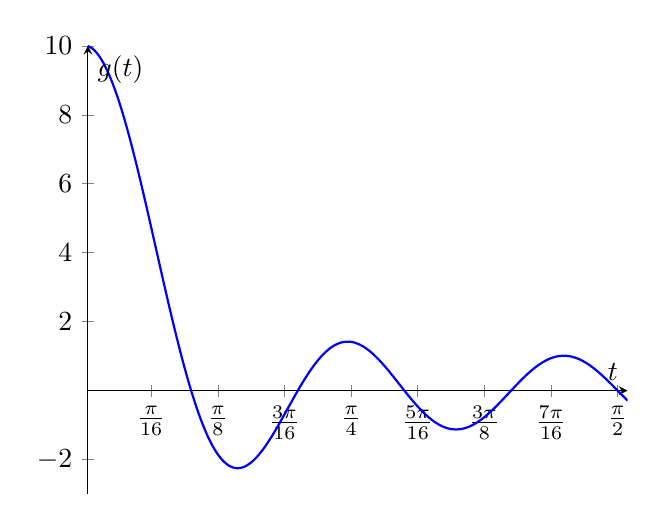
\begin{tikzpicture}%
                \begin{axis}[
                        axis lines = center,
                        xlabel = $t$,
                        ylabel = $g(t)$,
                        ymax=10,
                        ymin=-3,
                        xtick={0.0,
                                0.19634954084936207,
                                0.39269908169872414,
                                0.5890486225480862,
                                0.7853981633974483,
                                0.9817477042468103,
                                1.1780972450961724,
                                1.3744467859455345,
                                1.5707963267948966},
                        xticklabels={
                                $0$,
                                $\frac{\pi}{16}$,
                                $\frac{\pi}{8}$,
                                $\frac{3\pi}{16}$,
                                $\frac{\pi}{4}$,
                                $\frac{5\pi}{16}$,
                                $\frac{3\pi}{8}$,
                                $\frac{7\pi}{16}$,
                                $\frac{\pi}{2}$
                            }
                    ]
                    \addplot[blue, thick, samples=1000, domain=0.01:1.6] {(sin(10*deg(x)))/(sin(deg(x)))};
                \end{axis}
            \end{tikzpicture}}
    \end{center}

    Заметим вот что:

    \[
        \max_{[0, \pi/2]} g(t) = g(0) = 10
    \]

    Разложим в ряд Тейлора:

    \[
        \begin{aligned}[t]
             & g(t) = \frac{10t-\frac{10^3t^3}{6} + O(t^5)}
            {t-\frac{t^3}{6}+O(t^5)} = 10 \cdot
            \frac{1-\frac{100}{6}t^2 + O(t^4)}{1-\frac{t^2}{6}+O(t^4)}
            =                                               \\ & 10\left(1-\frac{100}{6}t^2 + O(t^4)\right)
            \left(1 + \frac{t^2}{6} + O(t^4)\right)
            = 10 \left(1-\frac{33}{2}t^2 + O(t^4)\right)
        \end{aligned}
    \]

    Напишем $\ln g(t)$:

    \[
        \ln g(t) = \ln 10 + \ln \left(1 - \frac{33}{2}t^2
        + O(t^4)\right)
        = \ln 10 - \frac{33}{2}t^2 + O(t^4)
    \]

    Напишем $e^{k\ln g(t)}$:

    \[
        e^{k\ln g(t)} = e^{k\ln 10}\cdot e^{-\frac{33}{2}kt^2}
        e^{O(t^4k)} = 10^k e^{-\frac{33}{2}kt^2} e^{O(t^4k)}
    \]

    Теперь считаем наш интеграл, разобьём на несколько частей
    ($\ve$ выберем потом):

    \[
        \int\limits_0^{\pi/2} =
        \int\limits_0^{\ve} + \int\limits_{\ve}^{\pi/10} + \int\limits_{\pi/10}^{\pi/2}
    \]

    Считаем первый интеграл:

    \[
        \int\limits_0^\ve e^{k\ln g(t)} dt =
        10^k \int\limits_0^\ve e^{-\frac{33}{2}kt^2} e^{O(k\ve^4)} dt = (*)
    \]

    Хотим вытащить $e^{O(k\ve^4)}$ наружу, для этого хотим чтобы
    $k\ve^4 \to 0$, тогда $e^{O(k\ve^4)} \sim 1$

    \[
        (*) \sim 10^k \int\limits_0^\ve e^{-\frac{33}{2}kt^2} dt
    \]

    Делаем замену $s = \sqrt{33k}t$.

    \[
        (*) = 10^k \int\limits_{0}^{\ve \sqrt{33k}}
        e^{-s^2/2} \frac{ds}{\sqrt{33k}}
        = \frac{10^k}{\sqrt{33k}}
        \int\limits_{0}^{\ve \sqrt{33k}}
        e^{-s^2/2} ds
    \]

    Если $\ve\sqrt{k} \to +\infty$, то

    \[
        (*) \sim \frac{10^k}{\sqrt{33k}} \cdot \sqrt{\frac{\pi}{2}}
    \]

    У нас есть два ограничения на $\ve$, можно допустим
    взять $\ve = k^{-1/3}$. Теперь давайте оценим хвосты.

    \[
        \int\limits_\ve^{\pi/10} \le \frac{\pi}{10} \max
        = \frac{\pi}{10} g(\ve)^k = \frac{\pi}{10} e^{k\ln g(\ve)}
        = \frac{\pi}{10} e^{k(\ln 10 - \frac{33}{2}\ve^2+O(\ve^4))}
        \sim \frac{\pi}{10} 10^k e^{-k\frac{33}{2}\ve^2}
        = o\left(\frac{10^k}{k}\right)
    \]

    И второй хвост:

    \[
        \int\limits_{\pi/10}^{\pi/2}
        \le \frac{\pi}{2} \cdot \left(\frac{1}{\sin \frac{\pi}{10}}\right)^k
        = o\left(\frac{10^k}{k}\right)
    \]

    Получается, что

    \[
        \int\limits_0^{\pi/2} \sim \int\limits_0^\ve
        \sim \frac{10^k}{\sqrt{33k}}\sqrt{\frac{\pi}{2}}
    \]

    Количество счастливых билетов растёт эквивалентно

    \[
        \frac{2}{\pi} \frac{10^{2k}}{\sqrt{132k}} \sqrt{\pi}
        = \frac{10^{2k}}{\sqrt{33\pi k}}
    \]

    $2k$ потому что в условии было $2k$ цифр а мы забыли про это.
\end{example}

\begin{example}[Метод Дарбу]

    Пусть $f(z) = \sum\limits_{n=0}^{+\infty} a_nz^n$ сходится
    в круге $\abs z < R$, тогда он сходится при
    $z = r$ если $0 < r < R$. Тогда $a_nr^n \to 0$,
    то есть $a_n = o(r^{-n})$,
    значит $a_n = o((R-\ve)^{-n})$.

    На границе круга сходимости есть особая точка,
    пусть она одна и это $a$.
    $g(z)$ имеет главную часть ряда Лорана
    в точке $a$ такую же как и функция $f$.
    Тогда у $f(z)-g(z)$ нет особой точки в $a$
    и (скорее всего) у $f-g$ больший круг сходимости.

    Если $g(z) = \sum\limits_{n=0}^{+\infty}
        b_nz^n$, то $(f-g)(z) = \sum\limits_{n=0}^{+\infty} (a_n-b_n) z^n$,
    или $a_n = b_n + o (\ldots)$.

    Посмотрим пример. Пусть $f(z) = \frac{\sqrt{2-z}}{(1-z)^2}$.
    Сходится в круге $\abs z < 1$, $z = 1$~--- особая точка.
    Можно взять $g(z) = \frac{1}{(1-z)^2}$.
    Единица в числителе потому что у $\sqrt{2-z} = 1$ при $z = 1$.

    \[
        f(z) - g(z) = \frac{\sqrt{2-z}-1}{(1-z)^2}
        = \frac{1-z}{(1-z)^2(1+\sqrt{2-z})}
        = \frac{1}{(1-z)(1+\sqrt{2-z})}
    \]

    Повторяем процесс: $h(z) = \frac{1}{2(1-z)}$.

    \[
        \begin{aligned}[t]
             & f(z) - g(z) - h(z) = \frac{1}{1-z}
            \left(\frac{1}{1+\sqrt{2-z}} - \frac{1}{2}\right)
            = \frac{1}{2(1-z)} \cdot \frac{2-(1+\sqrt{2-z})}{1+\sqrt{2-z}}
            =                                                \\
             & \frac{1}{2(1-z)} \cdot \frac{1}{1+\sqrt{2-z}}
            \cdot \frac{z-1}{1+\sqrt{2-z}}
            = -\frac{1}{2(1+\sqrt{2-z})^2}
        \end{aligned}
    \]

    Получилась функция, сходящаяся в круге $\abs z < 2$,
    а значит $c_n = o((2-\ve)^{-n})$. Подставим коэффиценты
    $f$ ($a_n$) исходя из следующей формулы:

    \[
        \frac{1}{(z-a)^m} = \sum\limits_{n=0}^{+\infty}
        C_{n+m-1}^{n}
        \left(\frac{z}{a} \right)^n
    \]

    Получается:

    \[
        a_n = C_{n+1}^n + \frac{1}{2}C_n^n + o((2-\ve)^{-n})
        = n + \frac{3}{2} + o((2-\ve)^{-n})
    \]
\end{example}
